%%%%%%%%%%%%%%%%%%%%%%%%%%%%%%%%%%%%%%%%%%%%%%%%%%%%%%%%%%%%%%%%%%%%%%
% CS637: Database-Backed Websites
% Copyright 2015 Pejman Ghorbanzade <mail@ghorbanzade.com>
% Creative Commons Attribution-ShareAlike 4.0 International License
% More info: https://bitbucket.org/ghorbanzade/umb-cs637-2015s
%%%%%%%%%%%%%%%%%%%%%%%%%%%%%%%%%%%%%%%%%%%%%%%%%%%%%%%%%%%%%%%%%%%%%%

\section*{Question 1}

Consider the variable \texttt{\$room\_preparing\_orders} in the code snippet given below. Answer the following questions based on model functions provided below.

\lstset{language=php}
\begin{lstlisting}
if ($action == 'student_welcome'|| $action == 'select_room') {
  try {
  $sizes = get_available_sizes();
  $toppings=  get_available_toppings();
  $room_preparing_orders=  get_preparing_orders_of_room($room);
  $room_baked_orders=  get_baked_orders_of_room($room);
  } catch (PDOException $e) {
    $error_message = $e->getMessage(); 
    include('../../errors/database_error.php');
    exit();
  }
  include('student_welcome.php');
}
\end{lstlisting}

\begin{enumerate}
\item Model function \texttt{get\_preparing\_orders\_of\_room(\$room)}
\begin{lstlisting}
function get_preparing_orders_of_room($room) {
    global $db;
    $query = 'SELECT * FROM pizza_orders where status=1 and room_number=:room';
    $statement = $db->prepare($query);
    $statement->bindValue(':room',$room);
    $statement->execute();
    $orders = $statement->fetchAll();
    $statement->closeCursor(); 
    $orders = add_toppings_to_orders($orders);
    return $orders;
}
\end{lstlisting}
\item Model function \texttt{add\_toppings\_to\_orders(\$orders)}
\begin{lstlisting}
function add_toppings_to_orders($orders) {
      for ($i=0; $i<count($orders);$i++) {
        $toppings = get_orders_toppings($orders[$i]['id']);
        $orders[$i]['toppings'] = $toppings; // add toppings to order 
    } 
    return $orders;
}
\end{lstlisting}
\item Model function \texttt{get\_orders\_toppings(\$order\_id)}
\begin{lstlisting}
function get_orders_toppings($order_id) {
    global $db;
    $query = 'select T.topping_name from toppings T,order_topping OT where OT.topping_id=T.id and OT.order_id=:order_id';
    $statement = $db->prepare($query);
    $statement->bindValue(':order_id',$order_id);
    $statement->execute();
    $toppings = $statement->fetchAll();
    $statement->closeCursor();
    return $toppings;
}
\end{lstlisting}
\end{enumerate}

\begin{enumerate}[label=(\alph*)]
\item Draw the data structure for \texttt{\$room\_preparing\_orders}. Assume two rows with two toppings and three toppings, respectively.

\item Write a fragment of PHP code to count the toppings across all the rows (maybe more than two) held in \texttt{\$room\_preparing\_orders}.
\end{enumerate}

\section*{Solution}

Based on provided model functions, the variable \$room\_preparing\_orders will be an associative array corresponding to the table resulting from the following MySQL query.
\lstset{language=SQL}
\begin{lstlisting}
SELECT PO.id, PO.size_id, PO.day, PO.status, T.topping_name
FROM pizza_orders PO, toppings T, order_topping OT
WHERE PO.status = 1
  AND PO.room_number = :room
  AND OT.topping_id = T.id
  AND PO.id = OT.order_id;
\end{lstlisting}

\begin{enumerate}[label=(\alph*)]
\item Data structure of the \texttt{\$room\_preparing\_orders} multi-dimensional array, holding to pizza orders with 2 and 3 toppings respectively, is given in Figure \ref{fig12}, in which cells numbers inside brackets represent their indices. Access to name of the first topping of the first item for instance is achieved by calling \texttt{\$room\_preparing\_orders[0][3][0]}. Noteworthy that \textit{order} and \textit{toppings} are for illustration and cannot be replaced with indices for fetching data.
\newpage
\begin{figure}[H]\centering
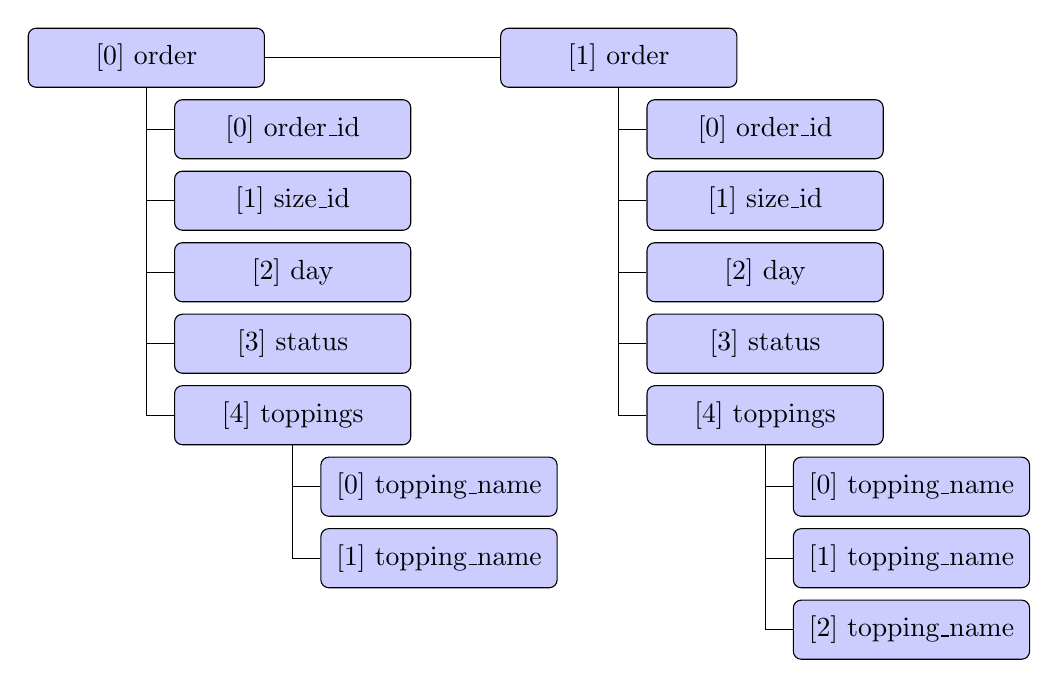
\begin{tikzpicture}[
  cell/.style={rectangle,draw,fill=blue!20,rounded corners=1mm,minimum width=3cm, minimum height=7.5mm},
  grandchild/.style={grow=down,xshift=1em,anchor=west, edge from parent path={(\tikzparentnode.south) |- (\tikzchildnode.west)}},
  first/.style={level distance=6ex},
  second/.style={level distance=12ex},
  third/.style={level distance=18ex},
  fourth/.style={level distance=24ex},
  fifth/.style={level distance=30ex},
  level 1/.style={sibling distance=6cm}
  ]
  \coordinate
  child[level distance=0mm] {
  node[cell, anchor=east] {[0] order}
    child[grandchild, first] {node[cell] {[0] order\_id}}
    child[grandchild, second] {node[cell] {[1] size\_id}}
    child[grandchild, third] {node[cell] {[2] day}}
    child[grandchild, fourth] {node[cell] {[3] status}}
    child[grandchild, fifth] {
    node[cell] {[4] toppings}
      child[grandchild, first] {node[cell] {[0] topping\_name}}
      child[grandchild, second] {node[cell] {[1] topping\_name}}
    }
  }
  child[level distance=0mm] {
  node[cell, anchor=east] {[1] order}
    child[grandchild, first] {node[cell] {[0] order\_id}}
    child[grandchild, second] {node[cell] {[1] size\_id}}
    child[grandchild, third] {node[cell] {[2] day}}
    child[grandchild, fourth] {node[cell] {[3] status}}
    child[grandchild, fifth] {
    node[cell] {[4] toppings}
      child[grandchild, first] {node[cell] {[0] topping\_name}}
      child[grandchild, second] {node[cell] {[1] topping\_name}}
      child[grandchild, third] {node[cell] {[2] topping\_name}}
    }
  };
\end{tikzpicture}
\caption{Data structure of \texttt{\$room\_preparing\_orders}}\label{fig12}
\end{figure}
\item The following code snippet in PHP counts the number of toppings for each row (order) of \texttt{\$room\_preparing\_orders} variable with arbitrary number of rows.

\lstset{language=php}
\begin{lstlisting}
for ($i = 0; $i < sizeof($room_preparing_orders); $i++) {
  $num_toppings[$i] = sizeof($room_preparing_orders[$i][4]);
}
echo implode($num_toppings);
\end{lstlisting}

\end{enumerate}

